\chapter{Statistical Mechanics} 
\label{chapter:stat-mech}

\section*{Objectives}
\begin{objectives}

\item Know the definitions of macrostates and microstates and
determine the number of microstates for a given macrostate
distribution of particles occupying energy levels.

\item Know what it means for a particular macrostate to be ``most likely.''

\item From graphs of energy distributions, determine which graphs
represent equilibrium distributions and of these which have higher
(lower) temperature.

\item Know the statistical definition of entropy in terms of the
number of microstates, $S = k \ln W$, and use this relation to calculate
the entropy of simple macroscopic distributions of particles among
energy levels.

\end{objectives}


\section{Introduction}

In this chapter we investigate a many particle system using
statistical principles to understand how energy is distributed among
the particles and what it means for a system to be in thermal
equilibrium.  Also we introduce a quantity called entropy and show how
changes in entropy lead a system toward thermal equilibrium.  Our
analysis, in terms of changes in entropy, of how thermal energy is
exchanged between two systems allows us to give a statistical
definition for temperature that is directly associated with our
physiological sensations of 'hot' and 'cold' and is consistent with
the kinetic definition which says that the temperature is proportional
to the average kinetic energy per particle in a system.
    
    
\section{Model for a System of Particles}
     
Here we develop a model for a system containing a large number of
particles, each of which can have one of a discrete set of
equally-spaced energies, or energy levels.  Our ultimate goal is to
determine the most likely distribution of the particles among the
energy levels; that is, if the levels are numbered 0, 1, 2, etc., we
want to find the average numbers of particles, $n_0$, $n_1$, $n_2$,
etc., that have each of the possible energies.  We'll find that this
average, or equilibrium, distribution is one in which the number of
particles with increasing energies forms a decreasing geometric
series.
    
The particles in our system are identical yet, in principle,
distinguishable.  What is meant by the seemingly contradictory phrase
'identical yet distinguishable' is the following.  Imagine that the
particles are manufactured with such precise uniformity that there is
no test which can be performed capable of distinguishing between any
two particles.  But to keep track of identity, we paint tiny numbers
on each one and only when we scrutinize very closely by examining the
numbers (i.e., we look at the system microscopically) are we able to
distinguish among the identical particles.  A more superficial
examination of the system wherein the tiny numbers are ignored is
called a macroscopic investigation of the system.
    
Any real system consists of a large number of particles, typically on
the order of $10^{23}$.  For now, we assume the system is isolated,
i.e., it cannot exchange either particles or energy with its
surroundings, so that the total number of particles and the total
energy are conserved.  Each particle can have only certain values of
energy, which are dictated by the system we are trying to model.  To
keep things as simple as possible, we use a model in which each
particle can have a specific energy among a set of uniformly spaced
energy values or levels as in Fig.~\ref{fig:levels_e3}.  In this model
a particle can only have energies given by one of these levels and
nothing in between.
    
The concept of discrete values of energy might appear strange given
what we know about classical mechanics, where a particle can have any
value of energy over some range.  The idea of discrete energy levels
comes from quantum physics where the energy of atomic systems is
quantized.
    
We want to determine how the particles in our isolated system are most
likely to be distributed among the allowed energy levels with a fixed
amount of total energy.  For example, Fig.~\ref{fig:levels_e3} shows a
set of uniformly spaced energy levels with a spacing of $\epsilon$
energy units.  A dot drawn on an allowed energy level represents a
particle with that energy.
          
\begin{figure}[tbp]
\begin{center}
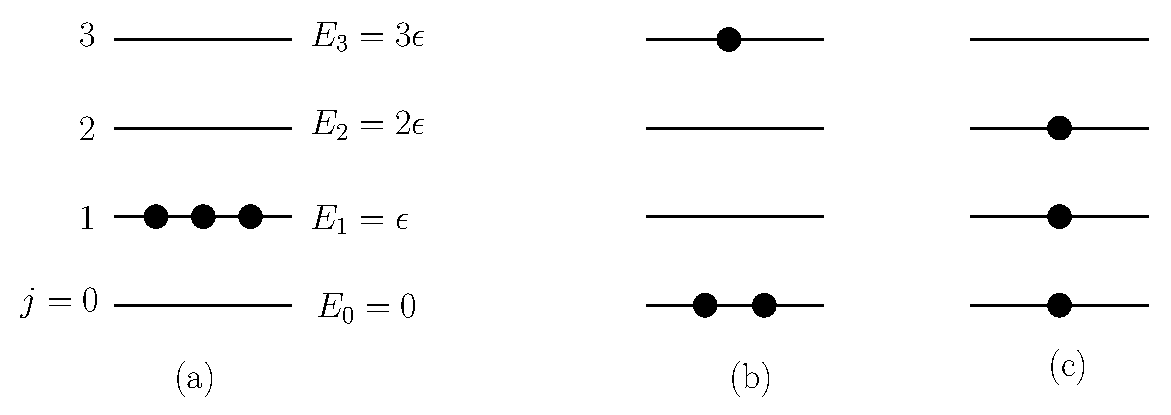
\includegraphics[width=4.3in]{statistical_mechanics/levels_e3.eps}
\end{center}
\caption{Energy levels populated by three particles with total energy 
$E = 3\epsilon$}
\label{fig:levels_e3}
\end{figure}     
     
Figure \ref{fig:levels_e3}(a) represents the special case where all
three particles have the same energy.  But there are other ways to
distribute the particles such that the total energy remains
$3\epsilon$, such as those given in figures \ref{fig:levels_e3}(b) and
\ref{fig:levels_e3}(c).  With a little thought you should be able to
see that for this three-particle example the three distributions of
Fig.~\ref{fig:levels_e3} are all that are possible such that the total
energy is fixed at $3\epsilon$.
        
We refer to each of the three distributions in
Fig.~\ref{fig:levels_e3} as a {\em macrostate} of the system since the
figure does not distinguish which of the three particles occupy a
given energy level.  A macrostate tells us {\em how many} particles
have a certain amount of energy and {\em not which ones} specifically.
But if we label the three particles `a', `b', `c', and then specify
which labeled particles are in which energy levels, that specification
is called a {\em microstate}.  For example, in
Fig.~\ref{fig:levels_e3}(c) there are six ways of arranging the three
labeled particles that result in the same macroscopic distribution.
In other words, six possible microstates yield the macrostate of
Fig.~\ref{fig:levels_e3}(c).  The number of microstates is six because
we can choose the particle in the $j = 0$ state in three ways, and for
each of these we can choose the particle in the $j = 1$ state in two
ways.  Multiplying, we find $3 \times 2 = 6$ ways to arrange the
particles.
        
To summarize:
        
\boxittext{A {\em macrostate} description of the distribution of 
particles specifies {\em how many} particles occupy each energy
level.
\vspace{0.2in}

A {\em microstate} description of the distribution of particles
specifies {\em which} particles occupy each energy level.}
        
Generally, macroscopic properties such as pressure, temperature,
energy, etc., are determined from the macrostate description of the
system.  Microstates belonging to each macrostate are experimentally
indistinguishable from one another since the macroscopic properties
are the same for all the microstates.  The real significance in
enumerating all the microstates is related to determining how likely
it is for a given macrostate distribution of the energy to occur.
       

\section{Determining the Number of Microstates}
  
We now show how to calculate the total number of microstates that
belong to a macrostate.  To be general, we examine an isolated system
of $N$ particles with total energy $E$.  We denote the number of particles
in each level by the symbol $n_j$ where $j$ is an index referring to
different energy levels ($j = 0, 1, 2,\dots$).  Since we assume the energy
levels to be uniformly spaced, the energy of the $j^{\rm th}$ level may be
expressed as $E_j = j\epsilon$.  With this terminology the total number of
particles and the total energy can be written as
\begin{equation}
N = \sum_{j=0}^\infty n_j\text{\hspace{0.25in}and\hspace{0.25in}}
E = \sum_{j=0}^\infty n_jE_j.
\end{equation}
Because our system is isolated, and thus cannot exchange particles or
energy with its surroundings, $N$ and $E$ are constant.

A macrostate description of the distribution of particles among energy
levels specifies the set of numbers $\{n_0, n_1, n_2,\dots\}$, i.e.,
the number of particles in each energy level.  For example,
Fig.~\ref{fig:levels_e3}(b) corresponds to the macrostate $\{2, 0, 0, 1,
0, 0, \dots\}$.

For a given macrostate, the number of microstates is the number of
ways of arranging the $N$ particles among the energy levels such that $n_0$
particles are in level 0, $n_1$ are in level 1, etc.  The result of a
combinatorial analysis for the number of microstates $W$ is

\begin{boxiteq}
{
\begin{equation}
W = \frac{N!}{n_0!\,n_1!\,n_2!\,n_3!\,\dots},
\label{eq:w}
\end{equation}
}
\end{boxiteq}
\vspace{-.3in}

\begin{large}
\begin{center}
number of microstates\\
in a macrostate
\end{center}
\end{large}

\noindent where we use the symbol ``!'' to denote a factorial product
(i.e.  $3! = 3\times2\times 1 = 6$), with $0!$ Being defined as 1.
Returning to the macrostate of Fig.~\ref{fig:levels_e3}(b) we
calculate the number of microstates to be $W = 3!/(2!0!0!1!) = 3$.
Hence there are three ways of arranging the distribution shown in
figure \ref{fig:levels_e3}(b).

A fundamental assumption of statistical mechanics is that no
microstate is more likely to occur than any other.  That is, {\em all
microstates are equally likely}.  But not all {\em macrostates} have
the same number of microstates.  This is a very important idea.  Since
each microstate has the same probability of occurring, the macrostate
having the greatest number of microstates is the most likely
macrostate.  In other words, the distribution $\{n_0, n_1,
n_2,\dots\}$, for which $W$ in Eq.~(\ref{eq:w}) assumes its greatest
value is the most likely distribution of particles among energy
levels.  

%For a system in a macrostate which is not the most likely macrostate,
%subsequent internal redistributions of the energy among particles take
%the system, on average, to macrostates which are more likely (i.e.,
%have larger values of $W$).  How does the system know how to do this?
%As the following example illustrates, this behavior is based entirely
%on the interactions between randomly selected pairs of particles in
%which energy is transferred from one particle to the other.
  

%\begin{example}{\label{ex:macro4-6}
%{\bf Statistical basis for a system of particles evolving to the most
%likely macrostate.}  Show, for a system in a macrostate that is not
%likely macrostate, that a two-particle collision, on average, takes
%the system to a more likely macrostate.  Specifically, consider
%macrostate $\{1, 2, 0, 0, 1, \dots\}$ labeled D in
%Fig.~\ref{fig:macro4-6}, in a system of 4 particles with 6 units of
%energy.
%\begin{figure}[t]
%\begin{center}
%\scalebox{0.4 }{\includegraphics{statistical_mechanics/macro4-6.eps}}
%\end{center}
%\caption{Possible macrostates for a system of $N = 4$ particles having
%total energy $E = 6$.}
%\label{fig:macro4-6}
%\end{figure}   
%} {Figure \ref{fig:macro4-6} shows all possible macrostates for a
%system of $N = 4$ particles with total energy $E = 6$.  The macrostates
%are labeled A through I with the total number of associated
%microstates $W$ for each macrostate (calculated from Eq.~(\ref{eq:w}) given
%beneath the level diagram.
%
%
%\begin{table}[h]
%\caption{Macrostate of the system after transfer of one unit of energy
%in one collision starting in macrostate D.}
%\label{table:exchange}
%%\vspace{0.1in}
%\begin{center}
%\begin{tabular}{|c|c||c|c|} \hline   
%Collision & Final  & Collision &  Final  \\  
%Partners  & Macrostate & Partners & Macrostate \\\hline\hline
%(a,b) &  F &  (b,a) & B \\ \hline
%(a,c) &  F &  (c,a) & B \\ \hline
%(a,d) &  G &  (d,a) & --- \\ \hline
%(b,c) &  C &  (c,b) & C  \\ \hline
%(b,d) &  D &  (d,b) & --- \\ \hline
%(c,d) &  D &  (d,c) & --- \\ \hline
%\end{tabular}
%\end{center}
%\end{table}
%
%
%Table~\ref{table:exchange} shows the possible outcomes of all the
%collisions between pairs of particles in macrostate D in which one
%unit of energy is exchanged.  The notation (b,d) in the table means
%particles b and d collide, with one unit of energy transferred {\em
%from} b {\em to} d.  On the other hand (d,b) is a collision between
%the same two particles with the energy now transferred {\em from} d
%{\em to} b.  For each collision the macrostate of the system after the
%collision is given.  (The table entry ``---'' means this collision is
%not allowed because it would require a particle to have energy less
%than the lowest energy level).
%
%We notice from Table~\ref{table:exchange} that out of the nine
%possible collisions, eight of these take the system to a macrostate
%whose value of $W$ is equal to or greater than that of macrostate D.
%In other words, there is a probability of only 1/9 that the system
%starting in macrostate D goes to a macrostate which is less likely.
%Homework problem \ref{prob:macro4-6} asks you to perform a similar analysis
%starting from different macrostates in Fig.~\ref{fig:macro4-6}.
%     
%This example illustrates the statistical basis upon which a system
%evolves spontaneously from less likely to more likely macrostates.
%}     
%\end{example}

%As a system evolves, it is in a continual state of fluctuation, moving
%from macrostate to macrostate.  The system proceeds spontaneously
%through various macrostates with increasing values of $W$ toward the
%macrostate with the greatest number of microstates, $W_{\rm max}$.  A
%graph illustrating this trend in a system
%might look like that of Fig.~\ref{fig:w-increase}.  Note that because 
%$W$ can get very large (and for other reasons that we will discuss in 
%Section \ref{sec:entropy-def}), we plot the natural log of $W$ vs.\ time,
%rather than $W$ itself vs.\ time.
%
%\begin{figure}[h]
%\begin{center}
%\scalebox{0.6}{\includegraphics{statistical_mechanics/w-increase.eps}}
%\end{center}
%\caption{Variation in the natural log of the number of microstates as
%a system approaches equilibrium through a series of macrostates.}
%\label{fig:w-increase}
%\end{figure}
%
%
%Occasionally, as the system approaches its most likely macrostate a
%distribution with a smaller value of $W$ occurs, but this is short
%lived.  Furthermore, even after reaching the most probable macrostate,
%the system performs a `dance' wherein it spontaneously and randomly
%jumps to other macrostates.  For any real system these fluctuations in
%the distribution result in extremely small fractional changes in the
%value of $W$, so that $W$ always remains close to $W_{\rm max}$. When
%the system has reached the situation of hovering near the most likely
%macrostate, we say that the system is in {\em statistical equilibrium}, 
%or {\em thermal equilibrium}.

\section[Most Probable Macrostate]{Analytical Expression for the Most 
Probable Macrostate}
\label{sec:analytical}
Now that we know that there is a most probable macrostate, what is the
'shape' of its distribution?  That is, how are the particles
distributed among the energy levels in the most likely distribution?
Although we have considered examples with very few particles for
calculational convenience, we are really interested in larger numbers.

Consider the distribution in Fig.~\ref{fig:nonequilib}, in which there
are 2002 particles in the lowest energy level, 1002 in the next higher
level and 102 in the next.  Although higher energy levels are also
populated we are not interested in those numbers for the moment.  The
number of microstates for this particular macrostate is given by
\begin{equation}
W = \frac{N!}{2002!\,1002!\,102!\,n_3!\,n_4!\,\dots}.
\end{equation}

\begin{figure}[b]
\begin{center}
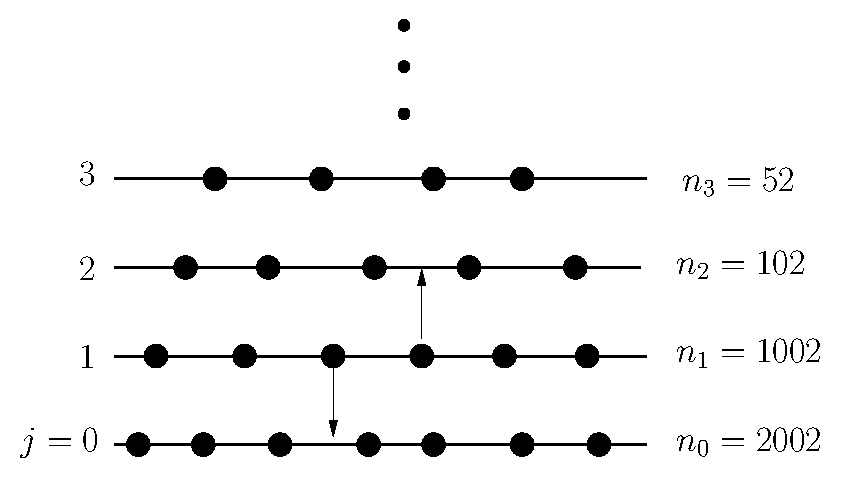
\includegraphics[width=3in]{statistical_mechanics/nonequilib.eps}
\end{center}
\caption{A typical nonequilibrium distribution.}
\label{fig:nonequilib}
\end{figure}

What happens to the value of $W$ if two particles from state $j = 1$
collide and transfer one unit of energy, one gaining energy $\epsilon$
and going to state $j = 2$, the other losing energy $\epsilon$ and
going to state $j = 0$, thus conserving energy?  The number of
microstates for this new macrostate is
\begin{equation}
W^\prime = \frac{N!}{2003!\,1000!\,103!\,n_3!\,n_4!\,\dots}.
\end{equation}
The ratio of these two values of $W$ yields
\begin{eqnarray}
\frac{W^\prime}{W} &=& \frac{N!}{2003!\,1000!\,103!\,n_3!\,n_4!\,\dots}\times 
                       \frac{2002!\,1002!\,102!\,n_3!\,n_4!\,\dots}{N!} 
                                   \nonumber \\
                   &=& \frac{1002\times 1001}{2003\times 103}\nonumber \\
                   &\simeq& 4.86 
\label{eq:w-ratio}
\end{eqnarray}
Thus we've shown that the macrostate of Fig.~\ref{fig:nonequilib} is
not the equilibrium macrostate because the ratio in
Eq.~(\ref{eq:w-ratio}) shows that $W^\prime$ (after the collision) is
significantly greater than $W$.

How do we know when a system has arrived at its most likely
macrostate?  If we can find a macrostate such that an exchange of
energy between two particles in a collision leaves $W$ practically
unchanged (i.e. $W^\prime/W \simeq 1$) then we can say the system is
in thermal equilibrium.

For example, consider a macrostate with 2142 particles in $j=0$,
722 in $j=1$, 242 in $j=2$, etc.  This macrostate has the same 
number of particles and the same total energy in levels 0, 1, and 2 as
the macrostate in Fig.~\ref{fig:nonequilib}.  Again we move two 
particles from $j=1$; one to $j=2$ and the other to $j=0$.  This 
time we find the ratio of the number of microstates to be 
\begin{eqnarray}
\frac{W^\prime}{W} &=& \frac{2142!\, 722!\, 242!}{2143!\, 720!\, 243!}
                               \nonumber \\
                   &=& \frac{722\times 721}{2143\times 243} \nonumber \\
                   &\simeq& 0.99964.
\end{eqnarray}
Here we see that the number of microstates stays very nearly the same,
decreasing by less that 0.04\%.  Thus in this case the system is in
thermal equilibrium because for a minor rearrangement of particles
among energy levels the number of possible microstates remains nearly
the same.

Let's generalize the ideas in the previous paragraphs.  If we 
have a macrostate with particle populations given by $\{ n_0, n_1, 
n_2, n_3, \dots\}$ and we switch two particles from level 1, one to level 2,
the other to level 0, then the ratio of the final number of 
microstates to the initial number is 
\begin{equation}
\frac{W^\prime}{W} = \frac{n_1(n_1-1)}{(n_0+1)(n_2+1)}. 
\end{equation}

The condition for statistical equilibrium is that $W^\prime/W \simeq 1$, 
which says that $W$ doesn't change appreciably after the two particles
are switched.  Now if we are talking about values of $n_j$ which are 
very large (say on the order of $10^6$) then a reasonable approximation 
is to set $n_j\pm 1 \simeq n_j$.  Therefore
\begin{equation}
\frac{W^\prime}{W} = \frac{n_1(n_1-1)}{(n_0+1)(n_2+1)}
                   \simeq \frac{n_1^2}{n_0 n_2} = 1, 
\end{equation}
or equivalently
\begin{equation}
\frac{n_1}{n_0} = \frac{n_2}{n_1}.
\end{equation}
This result implies that for a system with equally spaced energy 
levels, at equilibrium, the ratio of the number of particles in 
each level to the number in the level below is the same for all 
levels.  That is,
\begin{equation}
\frac{n_1}{n_0} = \frac{n_2}{n_1}=  \frac{n_3}{n_2}= \frac{n_4}{n_3} = \cdots
\end{equation}
That is, the ratios $n_3 /n_2$, $n_4 /n_3$, etc., are all equal to
$n_1/n_0$.  A series that has a constant ratio between successive
terms is known as a geometric series.  If we consider $n_j$ to be a
function of $j$, or $E_j$, then because the particle population decreases
with increasing energy levels, the form of the population function
must be a decreasing exponential of the form
\begin{equation}
n_j = n_0 e^{-\beta E_j}\text{\hspace{0.5in}}(j = 0, 1, 2,\dots, \infty).
\label{eq:boltz-dist}
\end{equation}
The positive constant $\beta$ determines how rapidly the population
function decreases with increasing energy.  The actual value of
$\beta$ depends on the average energy per particle in the system and
in order to make a direct correspondence to what we learned in kinetic
theory, the value of $\beta$ is defined in terms of the absolute
Kelvin temperature $T$ of the system as
\begin{equation}
\beta = \frac{1}{kT},
\label{eq:beta}
\end{equation}
where $k$ is Boltzmann's constant.  The distribution as given in
Eq.~(\ref{eq:boltz-dist}) with $\beta$ as defined in
Eq.~(\ref{eq:beta}) is known as the Boltzmann distribution.
     

\begin{figure}[tbp]
\begin{center}
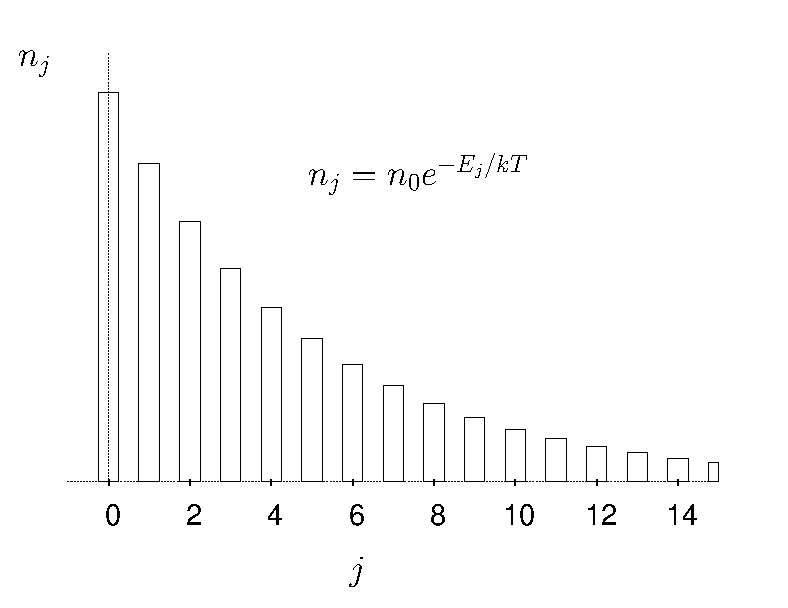
\includegraphics[width=3.8in]{statistical_mechanics/boltz-dist.eps}
\end{center}
\caption{The Boltzmann equilibrium distribution of particles among
energy levels.}
\label{fig:boltz-dist}
\end{figure}

In summary, we've shown that if a system of particles is distributed
among a set of allowed energy levels, then by randomly exchanging
energy within the system these particles ``seek'' a most probable
distribution which is the macrostate with the greatest number of
associated microstates.  When the system hovers near this distribution
the system is said to be in statistical, or thermal, equilibrium.  At
this point the macrostate fluctuates about a particle population which
has the form of a decreasing exponential function of the energy level
as shown in Fig.~\ref{fig:boltz-dist}.
     
     
\section{Microscopic Definition of Entropy}
\label{sec:entropy-def}

Now consider the problem of what happens to a system of particles if
we allow energy to be added to or removed from a system at
equilibrium.  We have discussed how energy may be transferred into or
out of a system by performing mechanical work either by compressing a
gas or allowing a gas to expand in a cylinder.  In the following
discussion however, we consider energy which flows from a `hotter'
object to a `colder' object, i.e., energy transferred via a temperature
difference.  This type of thermal energy transfer is often referred to
as heat flow.  Our goal is to show that there is an entropy change
associated with this process which is consistent with the definition
of entropy already discussed in our text.

First we show that the number of microstates $W$ changes when we allow
energy to enter or leave a system.  In the isolated systems we have
been considering, any internal redistribution of particles among
energy levels required that we move at least two particles.  But if
energy flows into a system from an external source, it is possible to
store that energy by changing the state of only one particle.  In such
a case, if we raise a particle from a level $E_j$ to a level $E_k$
(with $E_k> E_j$) increasing the energy of the system by an amount
$(k-j)\epsilon$, then using Eq.~(\ref{eq:w}) for the number of microstates,
we find that $W$ changes to a new value $W^\prime$ such that the ratio
$W^\prime/W$ is given by
\begin{equation}
\frac{W^\prime}{W} = \frac{n_j!\,n_k!}{(n_j-1)!\, (n_k+1)!} \simeq
 \frac{n_j}{n_k}
\label{eq:w-ratio2}
\end{equation}
using the approximation for large numbers of particles.
     
The significance of the result in Eq.~(\ref{eq:w-ratio2}) is that the number
of microstates increases ($W^\prime>W$) if we move a particle from a
more populated level to a less populated level (i.e., $n_j > n_k$) and
decreases ($W^\prime<W$) for the opposite case ($n_j < n_k$).
Moreover, if the system to which we are adding energy is in
statistical equilibrium, then the population of the energy levels is
given approximately by Eq.~(\ref{eq:boltz-dist}) and therefore
Eq.~(\ref{eq:w-ratio2}) may be further simplified to
\begin{eqnarray}
\frac{W^\prime}{W} &\simeq& \frac{n_j}{n_k} \nonumber \\
                   &=& \frac{n_0 e^{-E_j/(kT)}}{n_0 e^{-E_k/(kT)}} 
                                                  \nonumber \\
                   &=& e^{(E_k-E_j)/(kT)} \nonumber \\
                   &=& e^{Q/(kT)},
\label{eq:w-ratio3}
\end{eqnarray} 
where $Q = E_k - E_j$ is the amount of energy added to the system.
Eq.~(\ref{eq:w-ratio3}) shows that as a small amount of energy $Q$
flows into the system at equilibrium (small in order that the
distribution does not change drastically), then the change in $W$
depends only on how much energy is added and not on how many particles
are moved.  Taking the natural logarithm of both sides of
Eq.~(\ref{eq:w-ratio3}) we obtain
\begin{eqnarray}
\ln\left(\frac{W^\prime}{W}\right) &=& \ln W^\prime - \ln W \nonumber \\
                                   &=& \Delta(\ln W) \nonumber \\
                                   &=& \frac{Q}{kT},
\end{eqnarray}     
or rearranging terms
\begin{equation}
\Delta(k\ln W) = \frac{Q}{T}.
\label{eq:pre-entropy}
\end{equation}
     
The remarkable expression given in Eq.~(\ref{eq:pre-entropy}) relates
a microscopic quantity (the change in the number of microstates $W$)
to the macroscopic (i.e., physically measurable) quantities $Q$ and
$T$.  Eq.~(\ref{eq:pre-entropy}) implies that if a small amount of
energy $Q$ in the form of heat flows into (positive $Q$) or out of
(negative $Q$) a system at a temperature $T$, then the quantity $k \ln
W$ changes accordingly.  In direct analogy with our previous
definition for entropy $S$, we see that the right hand side of
Eq.~(\ref{eq:pre-entropy}) must be identified with the change in
entropy $\Delta S$ associated with the transfer of energy $Q$ at a
temperature $T$.  Thus we are lead to a new definition of entropy in
terms of the number of microstates associated with the macrostate of
the system:

\begin{boxiteq}
{
\begin{equation}
S = k \ln W.
\label{eq:entropy}
\end{equation}
}
\end{boxiteq}
\vspace{-.1in}

By virtue of this definition of entropy in terms of the number of
microstates $W$, we see that the entropy is only a function of the
distribution of the particles among energy levels and does not depend
on the process by which those levels were populated.  A quantity such
as this which does not depend on the history of the system is
called a state variable.  Changes in entropy can be measured in a
straightforward way by measuring the macroscopic quantities $Q$ and
$T$.  Thus, from Eqs.~(\ref{eq:pre-entropy}) and (\ref{eq:entropy}) we
have
\begin{equation}
\Delta S = \frac{Q}{T}.
\label{eq:deltaS}
\end{equation}


\begin{example}{Additivity of Entropy.}  
Show that the entropy of two isolated
systems, A and B, considered as one large system, is the sum of the
entropies $S_A$ and $S_B$ of the individual systems.

\solution
We use the fact that $W_{\rm tot}= W_A\times W_B$.  Taking the
logarithm of this expression we get
\begin{equation}
\ln W_{\rm tot} = \ln(W_A \times W_B) = \ln W_A + \ln W_B.
\end{equation}
Therefore, from Eq.~(\ref{eq:entropy}) we have
\begin{eqnarray}
S =k \ln W_{\rm tot} &=& k (\ln W_A + \ln W_B) \nonumber \\
  &=& S_A + S_B 
\end{eqnarray}
Thus if a system is composed of several subsystems, the total entropy
is the sum of the entropies of the individual subsystems.
\end{example}
  
As Eq.~(\ref{eq:deltaS}) points out, it is not the value of $S$ that
is of fundamental importance, but rather the change in entropy,
$\Delta S$.  Thus the role of entropy in thermodynamics is analogous
to the role of potential energy in classical mechanics, where the
behavior of a system depends on changes of potential energy, not on
its absolute value.

\begin{example}{Entropy Change Associated with the Spontaneous
    Exchange of Heat.}
\label{ex:deltaS}
A small amount of heat energy $Q$ flows from system A at temperature $T_A$
to system B at temperature $T_B$, where $T_A > T_B$.  Show that the 
entropy increases in such a process.
\solution
The entropy change of the combined systems A and B is given by
\begin{eqnarray}
\Delta S &=& \Delta S_A + \Delta S_B \nonumber \\
         &=& \frac{-Q}{T_A} + \frac{+Q}{T_B},
\label{eq:deltaS-ex}
\end{eqnarray}    
where $Q$ is taken as an intrinsically positive quantity.  Because
$T_A > T_B$, the negative entropy change $\Delta S_A$ is smaller in
magnitude than the positive entropy change $\Delta S_B$.  Thus $\Delta
S > 0$, and therefore when heat flows from A to B spontaneously, the
entropy of the combined systems increases.
\end{example}

The conclusion drawn in Example~\ref{ex:deltaS} makes sense since the
combined system is trying to move toward the maximum value of the
quantity $W_A\times W_B$.  Can you now understand why it is that you
never see energy flow spontaneously from a cooler object to a hotter
object?  Imagine a heat flow from system B to A such that $T_B < T_A$.
This time the signs attached to the $Q$'s in Eq.~(\ref{eq:deltaS-ex})
are reversed, making the total entropy change $\Delta S < 0$.  The
total entropy decreases when heat flows from a colder system to a
hotter system.  Therefore it seems that nature's principle of
increasing entropy is responsible for the one-way spontaneous flow of
heat.

\section*{Problems}
\markright{PROBLEMS}

\begin{problem}
  In a system of 10 particles and 15 units of energy, one of the
  macrostates consists of five particles in energy level 0, two
  particles in energy level 2, one particle in energy level 3, and two
  in energy level 4.  In other words, the macrostate is $\{5, 0, 2, 1,
  2, 0, \dots\}$.  Calculate the number of microstates in this
  macrostate.
  \label{prob:micro-calc}
\end{problem}
 
\begin{problem}
  For the system of 10 particles and 15 units of energy discussed in
  Problem \ref{prob:micro-calc}, identify another possible macrostate
  other than the one in the problem.  Use the curly bracket notation.
\end{problem}

\begin{problem}
  At the beginning of section \ref{sec:analytical}, two particles in
  the energy level $j = 1$ collided and transferred one unit of
  energy, thus moving the system to a new macrostate whose number of
  microstates $W^\prime$ is such that $W^\prime/W = 4.86$.  Starting
  from this new macrostate, move two more particles from level $j =1$
  to levels $j = 0$ and $j = 2$ and calculate the new ratio
  $W^\prime/W$.
  \label{prob:w_ratio}
\end{problem}
	
\begin{problem}
  At a certain instant of time a system of 4000 particles has the
  macrostate shown in the left side of Fig.~\ref{fig:levels_4000},
  i.e., the macrostate is 
  \[\{2000, 1700, 300, 0,\dots\}.\]  
  Two
  particles now leave the $j = 1$ state, one gaining energy and going
  to $j = 2$, the other losing energy and going to $j = 0$, thus
  resulting in the macrostate 
  \[\{2001, 1698, 301, 0,\dots\}\] 
  shown
  below right.  Is the system in equilibrium?  How can you tell?
  \label{prob:levels_4000}
  \begin{figure}[h]
\begin{center}
  \scalebox{0.6}{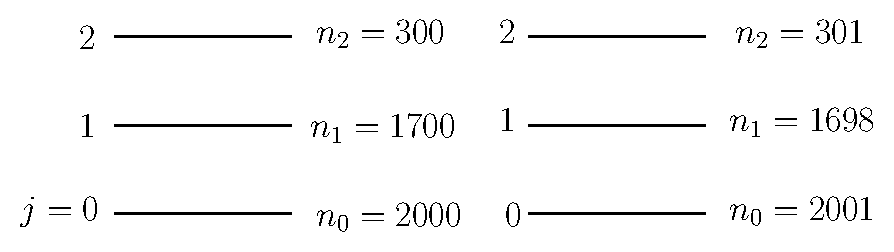
\includegraphics{statistical_mechanics/prob_4000.eps}}
\end{center}
\caption{For Problem \ref{prob:levels_4000}.}
\label{fig:levels_4000}
\end{figure}
\end{problem}


\begin{problem}
  For a system of uniformly spaced energy levels that has come to
  thermal equilibrium, the numbers of particles in levels 0 and 1 are
  observed to be 5000 and 4500, respectively.  Estimate the number of
  particles in level 2.
  \label{prob:equilibrium}
\end{problem}


\begin{problem}
  System A, which has the equilibrium macrostate 
  \[\{4000, 3800, 3610,3430, 3258,3095, \dots\},\] 
   is placed in thermal contact with another
  system B, which has the equilibrium macrostate 
  \[\{6000, 5580, 5189,4826, 4488, 4174, 3882, \dots\}\] 
   and the same energy level spacing
  as system A.
  \begin{enumerate}
  \item Which system is hotter, i.e., has a greater temperature?
  \item In which direction will energy tend to flow?
  \item Support your answer to part (b) with a calculation, for the
    case in which a particle in level 1 in system A exchanges 1 unit
    of energy with a particle in level 3 in system B.  Hint: Compare
    the values of the product, $W_AW_B$, before and after the exchange
    of energy.
  \end{enumerate}
  \label{prob:systemsAB}
\end{problem}


\begin{problem}
  The system in the macrostate $\{5, 0, 2, 1, 2, 0, \dots\}$ defined
  in problem \ref{prob:micro-calc} changes in the following way.  The
  particle in energy level 3 gives up one unit of energy to one of the
  particles in energy level 0.  Write the new macrostate in curly
  bracket notation.
  \label{prob:new_macrostate}
\end{problem}

\begin{problem}
  For the macrostate distributions of Figs.~\ref{fig:levels_e3}(a) and
  \ref{fig:levels_e3}(b),
  \begin{enumerate}
  \item Calculate the number of microstates $W$.
  \item Verify the values you calculated in part a) by making an
    exhaustive list of combinations of three distinguishable particles
    in energy levels such that the total energy is 3$\epsilon$.
  \end{enumerate}
  \label{prob:exhaustive_list}
\end{problem}



\begin{problem}
  A certain system is in the equilibrium macrostate 
  \[\{4000, 3800,3610, 3430, 3258, 3095, \dots\}.\]  
   Now one unit of energy is added,
  from outside the system, to one of the particles in energy level 2.
  \begin{enumerate}
  \item Write the new macrostate in the curly bracket notation.
  \item Show by direct computation that the number of microstates
    associated with the new macrostate is greater than the number of
    microstates associated with the original macrostate.
  \end{enumerate}
\end{problem}

\begin{problem}
  Consider a system of $N = 10^{20}$ particles occupying equally spaced
  energy levels.  The system is in thermal equilibrium at temperature
  $T = 290\units{K}$, and the level-spacing is $\epsilon =
  0.02\units{eV}$.
  \begin{enumerate}
  \item Calculate the Boltzmann factor, $e^{-\epsilon/kT}$.
  \item The system has $n_0 = 5.51 \times 10^{19}$ particles in the
    lowest level.  Determine $n_1$ and $n_2$.
  \item Now energy $\epsilon = 0.02\units{eV}$ is added to the system
    from outside, so that a single particle jumps up from level 1 to
    level 2.  Calculate $W_{\rm new}/W_{\rm old}$.
  \item Using your result from part c), calculate
    \[ \Delta S = S_{\rm new} - S_{\rm old} = k \ln W_{\rm new} - k
    \ln W_{\rm old} = k \ln (W_{\rm new}/W_{\rm old}) \] Express your
    answer in units of eV/K.
  \item Now calculate $\Delta S$ using the macroscopic form $\Delta S
    = Q/T$.  How do your results from parts d) and e) compare?
  \end{enumerate}
\end{problem}

\vspace{3in}
\noindent\textbf{Answers}
\vspace{3mm}

\noindent
{\bf \ref{prob:micro-calc}.}~$W = 7560$. 
{\bf \ref{prob:w_ratio}.}~$W^\prime/W = 4.79$.
{\bf \ref{prob:equilibrium}.}~$n_2 \simeq 4050$.
{\bf \ref{prob:systemsAB}.}~a)~A; b)~A to B; 
c)~$(W_A^\prime W_b^\prime)/(W_AW_B)~\simeq 1.02$.
{\bf \ref{prob:new_macrostate}.}~$\{ 4,1,3,0,2,0,\dots\}$.
{\bf \ref{prob:exhaustive_list}.}~a)~$W = 1$ for 
\ref{fig:levels_e3}(a), $W=3$ for \ref{fig:levels_e3}(b).
